\documentclass[a4paper]{article}
\usepackage[danish]{babel}
\usepackage[utf8]{inputenc}
\usepackage{amsmath} %Skal bruges for at kunne anvende matematik
\usepackage{graphicx} %Skal bruges for at kunne indsætte billeder

\begin{document}
\title{Boblesortering}
\author{
   Erik Vangslev, s185392
   \and
   Simon Gredal, s165017
   \and
   Jonas Kunert, s184231
   \and
   Steffen Cordes, s184208}
\date{11. oktober 2018}
\maketitle

\begin{abstract}
Dette dokument omhandler boblesortering. Der beskrives algoritmen og præsenteres en kompleksitetsanalyse.
\end{abstract}

\section{Introduktion}
Boblesortering \textit{(eng. bubble sort)} er en populær \textit{sorteringsalgoritme} og er en af de simpleste algoritmer at forstå og implementere. Dog er den ikke en særlig effektiv sorteringsalgoritme\footnote{Mere om dette i "Algoritmer og Datastrukturer 1"}; hverken for store eller små lister, og den anvendes sjældent i praksis. Boblesortering sorterer, som navnet antyder, elementerne i en liste ved at \textit{boble} hvert element gennem listen til sin rette plads i listen.

\subsection{Pseudokode}
Wikipedia \cite{WikiBubble} giver følgende pseudokode for boblesortering.

\begin{verbatim}
procedure bubbleSort( A : list of sortable items ) defined as:
  do
    swapped := false
    for each i in 0 to length(A) - 2 inclusive do:
      if A[i] > A[i+1] then
        swap( A[i], A[i+1] )
        swapped := true
      end if end for
    while swapped
end procedure
\end{verbatim}
En illustration af en kørsel af boblesortering fra Wikipedia kan ses på figur 1.

\section{Analyse af bobblesortering}
Antallet af sammenligninger, som boblesortering udfører på en tabel af længde \(n\),
er i værste fald
\[ 
\displaystyle\sum_{i=1}^{n-1} i = 1 + 2 + 3 + \cdots + n - 1 = \frac{n(n - 1)}{2}
\]
I bedste fald er antallet af \(n-1\). Se tabel 1.

\begin{figure}
	\centering
	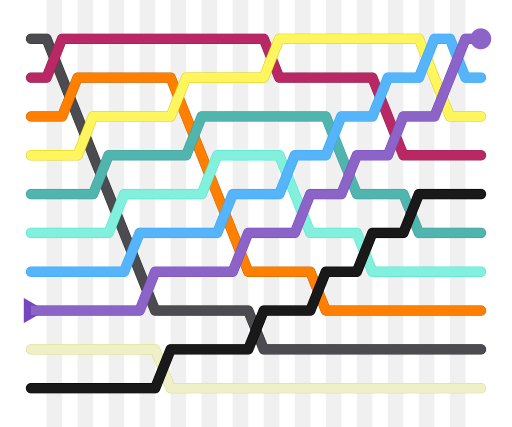
\includegraphics[width=0.4\linewidth]{Bubblesort.png}
	\caption{Illustration af boblesortering.}
\end{figure}

\begin{table}[h!]
	\begin{center}
		
		\label{tab:table1}
		\begin{tabular}{|c|l|} % <-- Alignments: 1st column left, 2nd middle and 3rd right, with vertical lines in between
			\hline
			\textbf{Værst} & \(n(n - 1)/2\)\\
			\hline
			\textbf{Bedst} & \(n-1\) \\
			\hline
		\end{tabular}
	
	\end{center}
	\caption{Antal sammenligninger for boblesortering.}
\end{table}



\begin{thebibliography}{99}

\bibitem{DonaldKnuthTAOCP}
  Donald Knuth.
  The Art of Computer Programming,
  Volume 3.
  Addison-Wesley

\bibitem{WikiBubble}
\begin{verbatim}
http://en.wikipedia.org/wiki/Bubble_sort
\end{verbatim}

\end{thebibliography}


\end{document}
